% Software Development for Mobile Devices
\documentclass[11pt,english,numbers=endperiod,parskip=half]{scrartcl}

\usepackage{color}
\usepackage{graphicx}
\usepackage{minted}
\usepackage{fancyhdr}
\usepackage{pdflscape}
\usepackage{listings}

\pagestyle{fancy}

\rhead{Daniel Parker - 971328X}
\lhead{COS30017 - Software Development for Mobile Devices}

\title{Assignment 08}
\subtitle{COS30017 - Software Development for Mobile Devices}
\author{Daniel Parker 971328X}

\date{\today}

\begin{document}
\maketitle
\thispagestyle{empty}

\section{Task 1}
\subsection{Introduction}
\subsection{Performance Optimisations}
The movie ratings app was particularly in need of optimisation, and this was due
to the size of the data being loaded and also how the java objects to visualise
them were being created. The observed issue is that when the user scrolls down
the list of movies, the list starts to jitter and lag while it tries to load the
upcoming movies. The cause of this problem is that view objects are being created
unnecessarily only to be thrown out milliseconds later. This also has the flow-on
effect of the java garbage collector having to clean up all the no-longer used
objects on the heap.

To solve this issue, the code has been modified slightly to reuse already allocated
View objects when possible, stopping the need for new objects to be created. In
code snippet [1] the convertView has been reused instead of allocating new View
objects. The other key addition has been to include the use of a ViewHolder, which
allows the app not to have to continuously run findViewById() which is an
expensive operation to perform many hundreds of times per second.



\subsection{Usability Improvement}
This app also suffered from an issue of the data set taking a while to load into
memory. Fixing this issue involved adding a progress dialog which displayed to
the user a spinner and notification that the app was loading the movie ratings.

This was achieved by using an AsyncTask which runs on a separate thread and posts
back when it has completed. The code snippets [2] and [3] show how this was achieved,
and the screenshot shows the result in the app.

\begin{figure}[H]
\centering{
	\fbox{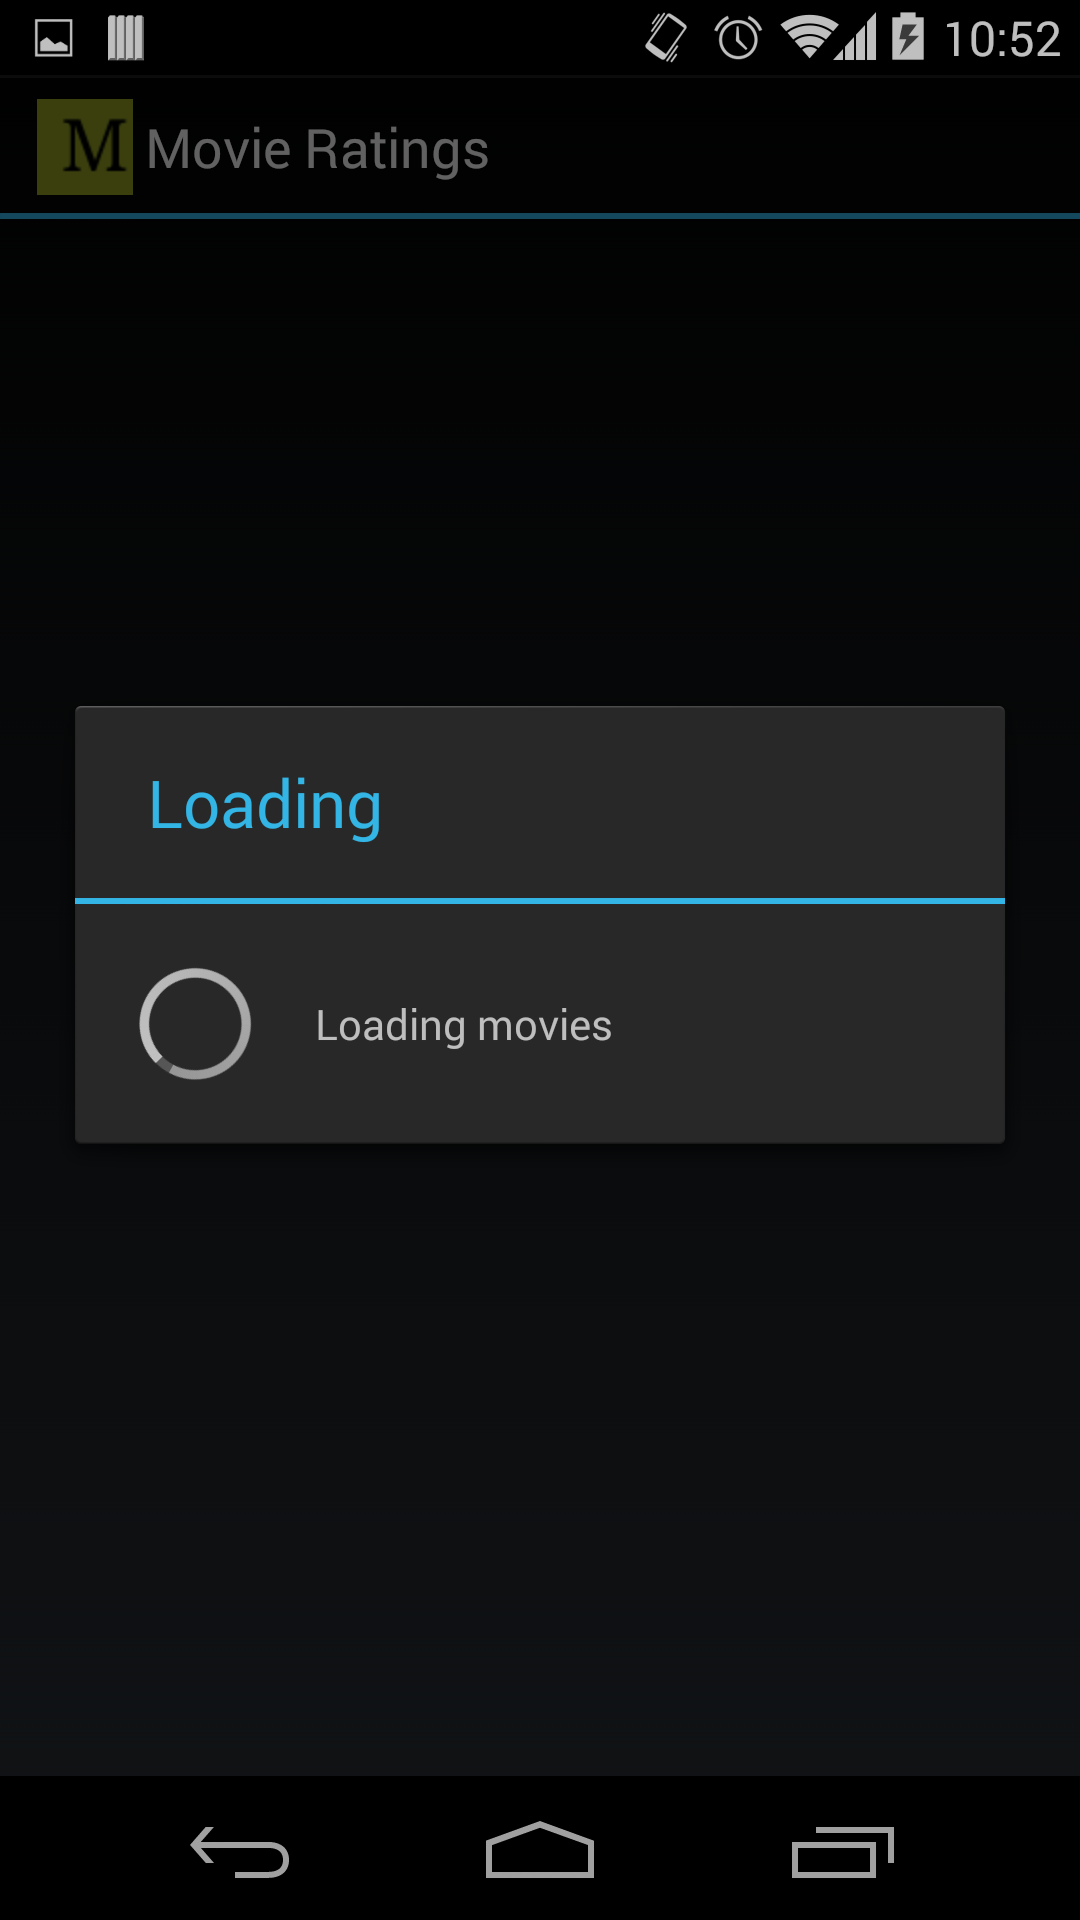
\includegraphics[width=5cm]{images/loading.png}}
}\\
\end{figure}

\subsection{References}
\begin{enumerate}
	\item{Making ListView Scrolling Smooth, \textit{Android Developers},
	viewed 28 October 2014,
	\textless http://developer.android.com/training/improving-layouts/smooth-scrolling.html\textgreater}
	\item{Vasa, R 2014, `Lecture 08 Enhancing Lists', \textit{Software Development for Mobile Devices},
	Learning materials on Blackboard, Swinburne University of Technology, 1 October, viewed 30 October 2014.}
\end{enumerate}

\begin{landscape}
\subsection{Appendix}
\subsubsection{1}
\inputminted[firstline=64, lastline=94, frame=single]{java}{../../Apps/MovieRatings/app/src/main/java/swin/examples/MovieRatingsActivity.java}
\subsubsection{2}
\inputminted[firstline=45, lastline=51, frame=single]{java}{../../Apps/MovieRatings/app/src/main/java/swin/examples/MovieRatingsActivity.java}
\subsubsection{3}
\inputminted[firstline=164, lastline=190, frame=single]{java}{../../Apps/MovieRatings/app/src/main/java/swin/examples/MovieRatingsActivity.java}
\end{landscape}
\section{Task 2}
This improved suntime app contains various new features including custom locations
using a map, sun rise and set times for a range of dates, and share functionality
to send a specific day's sun rise and set times for a location.

The new app includes the following fragments:
\begin{itemize}
	\item{List of preset locations}
	\item{Custom location using map}
\end{itemize}

\subsection{Screenshots}
\setlength\fboxsep{0pt}
\setlength\fboxrule{0.5pt}

\begin{figure}[H]
\centering{
	\fbox{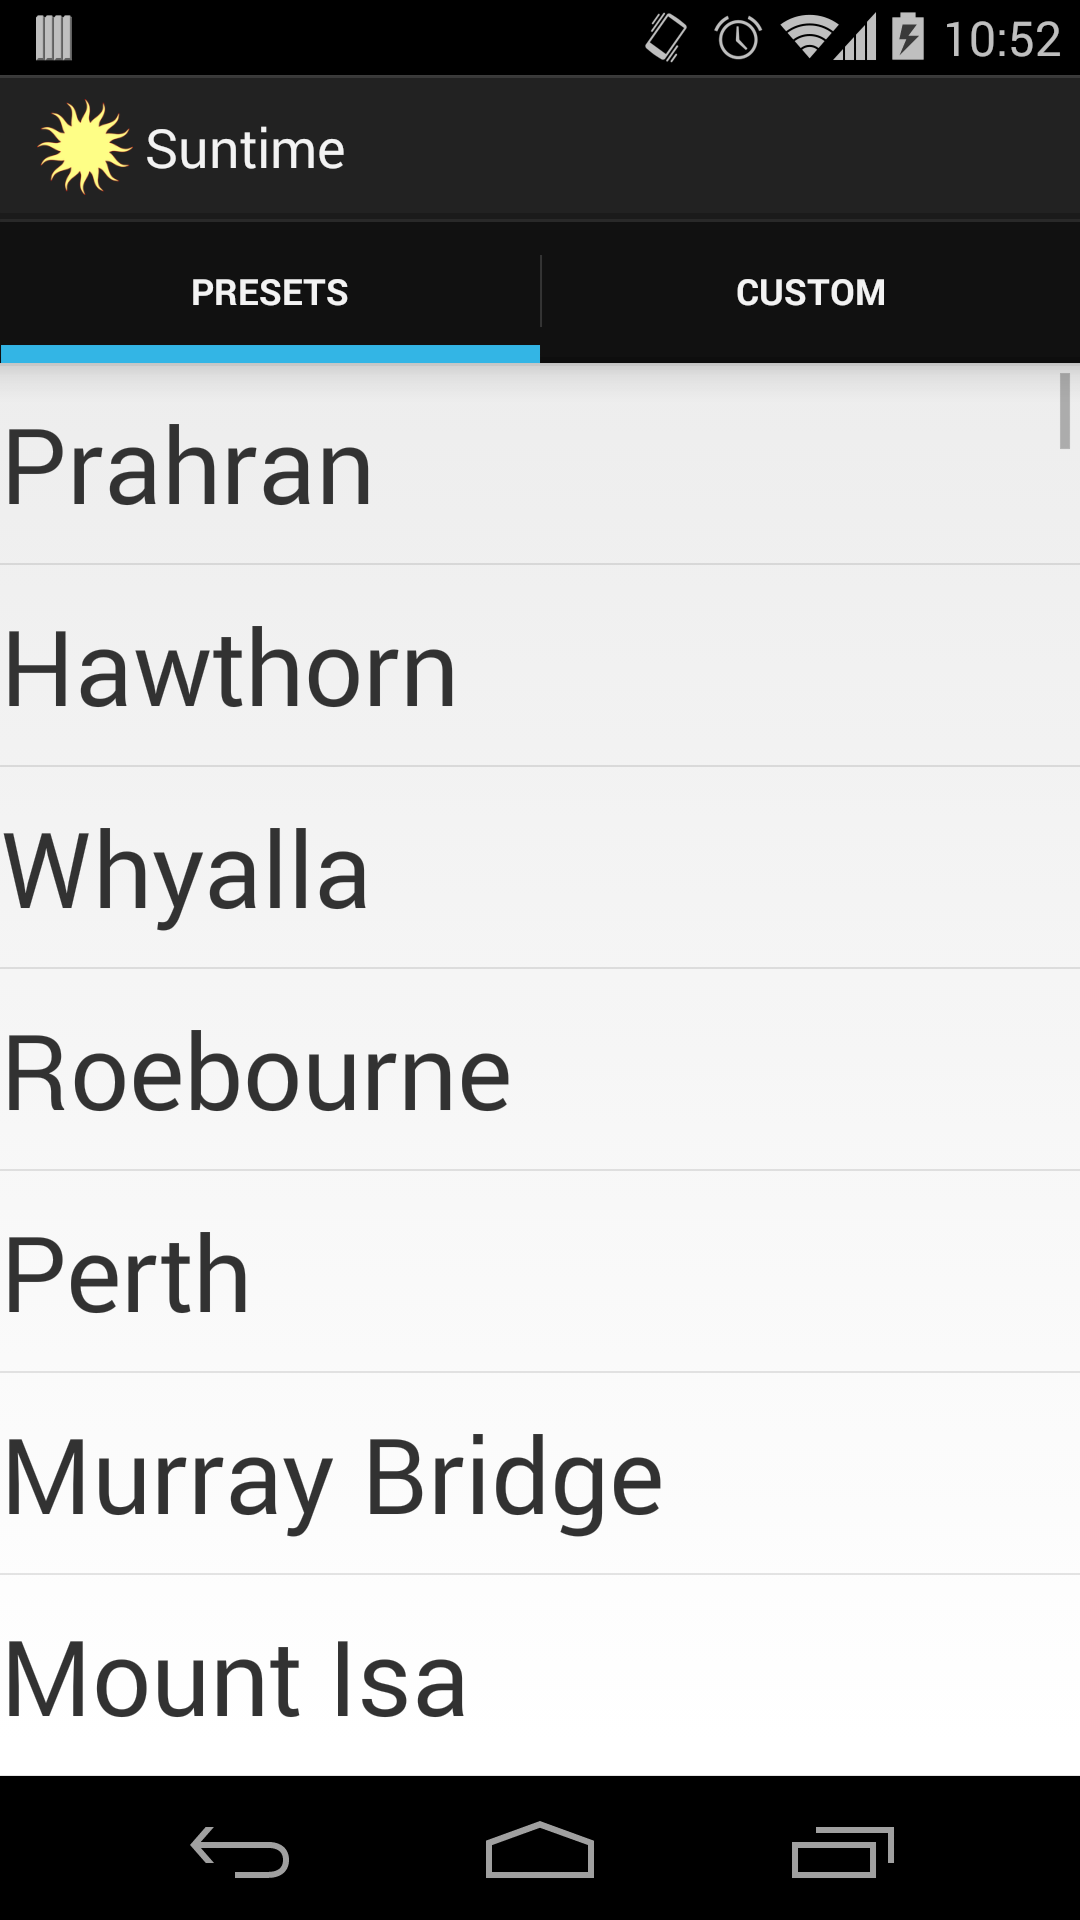
\includegraphics[width=5cm]{images/preset.png}}
}\\
\end{figure}

\begin{figure}[H]
\centering{
	\fbox{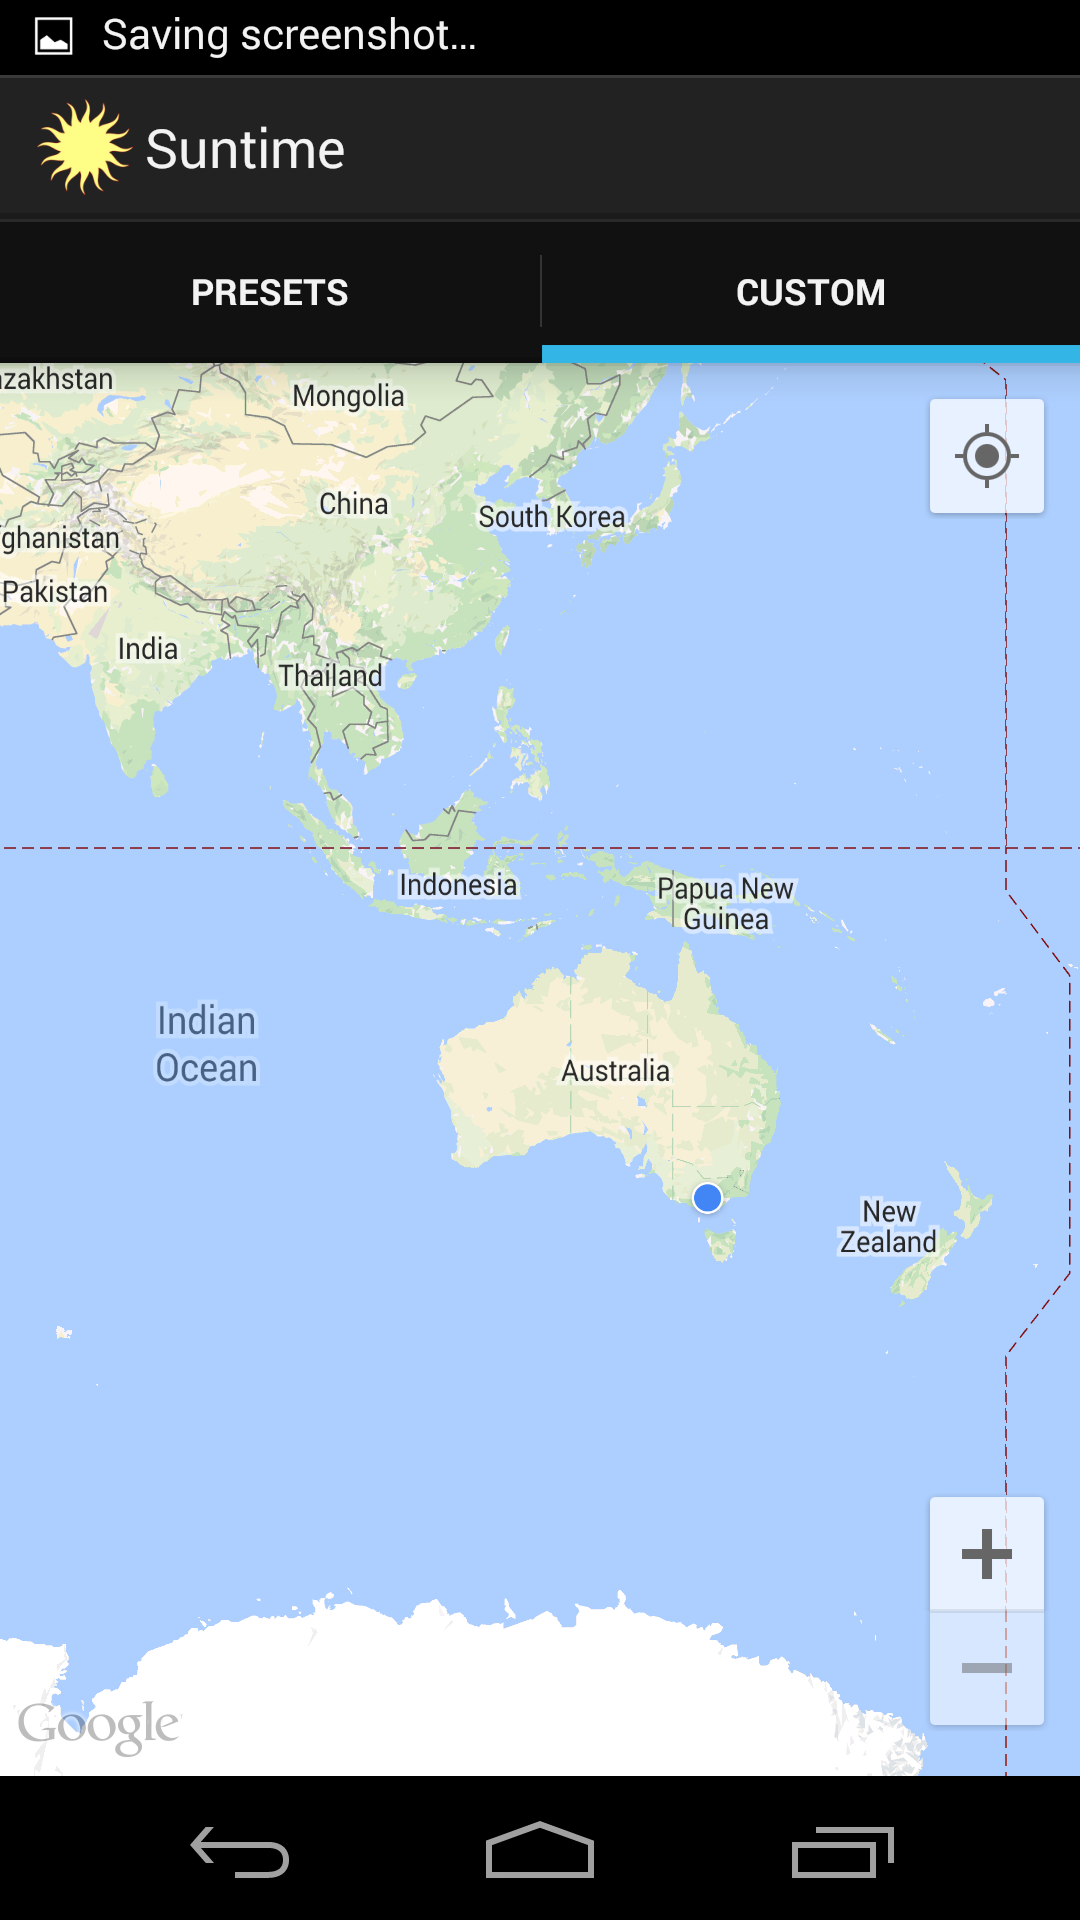
\includegraphics[width=5cm]{images/map.png}}
}\\
\end{figure}

\begin{figure}[H]
\centering{
	\fbox{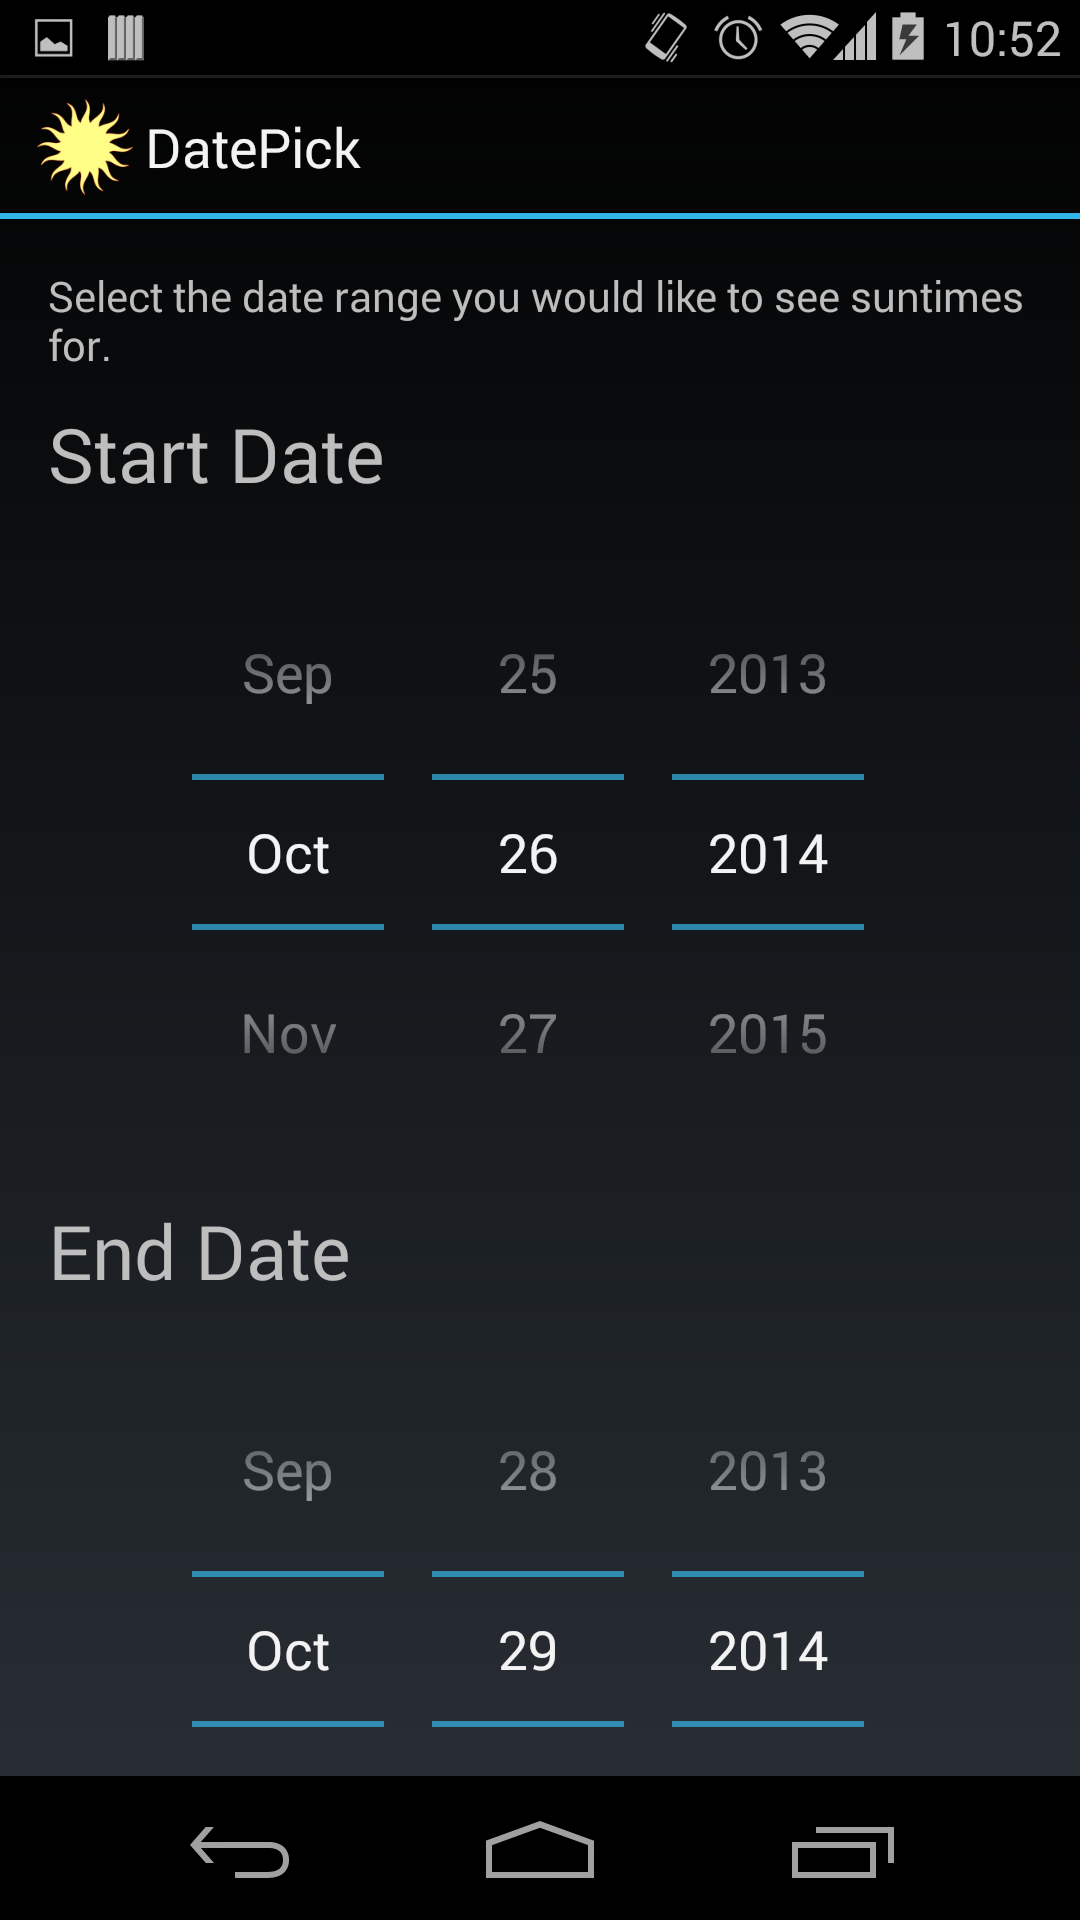
\includegraphics[width=5cm]{images/range.png}}
}\\
\end{figure}

\begin{figure}[H]
\centering{
	\fbox{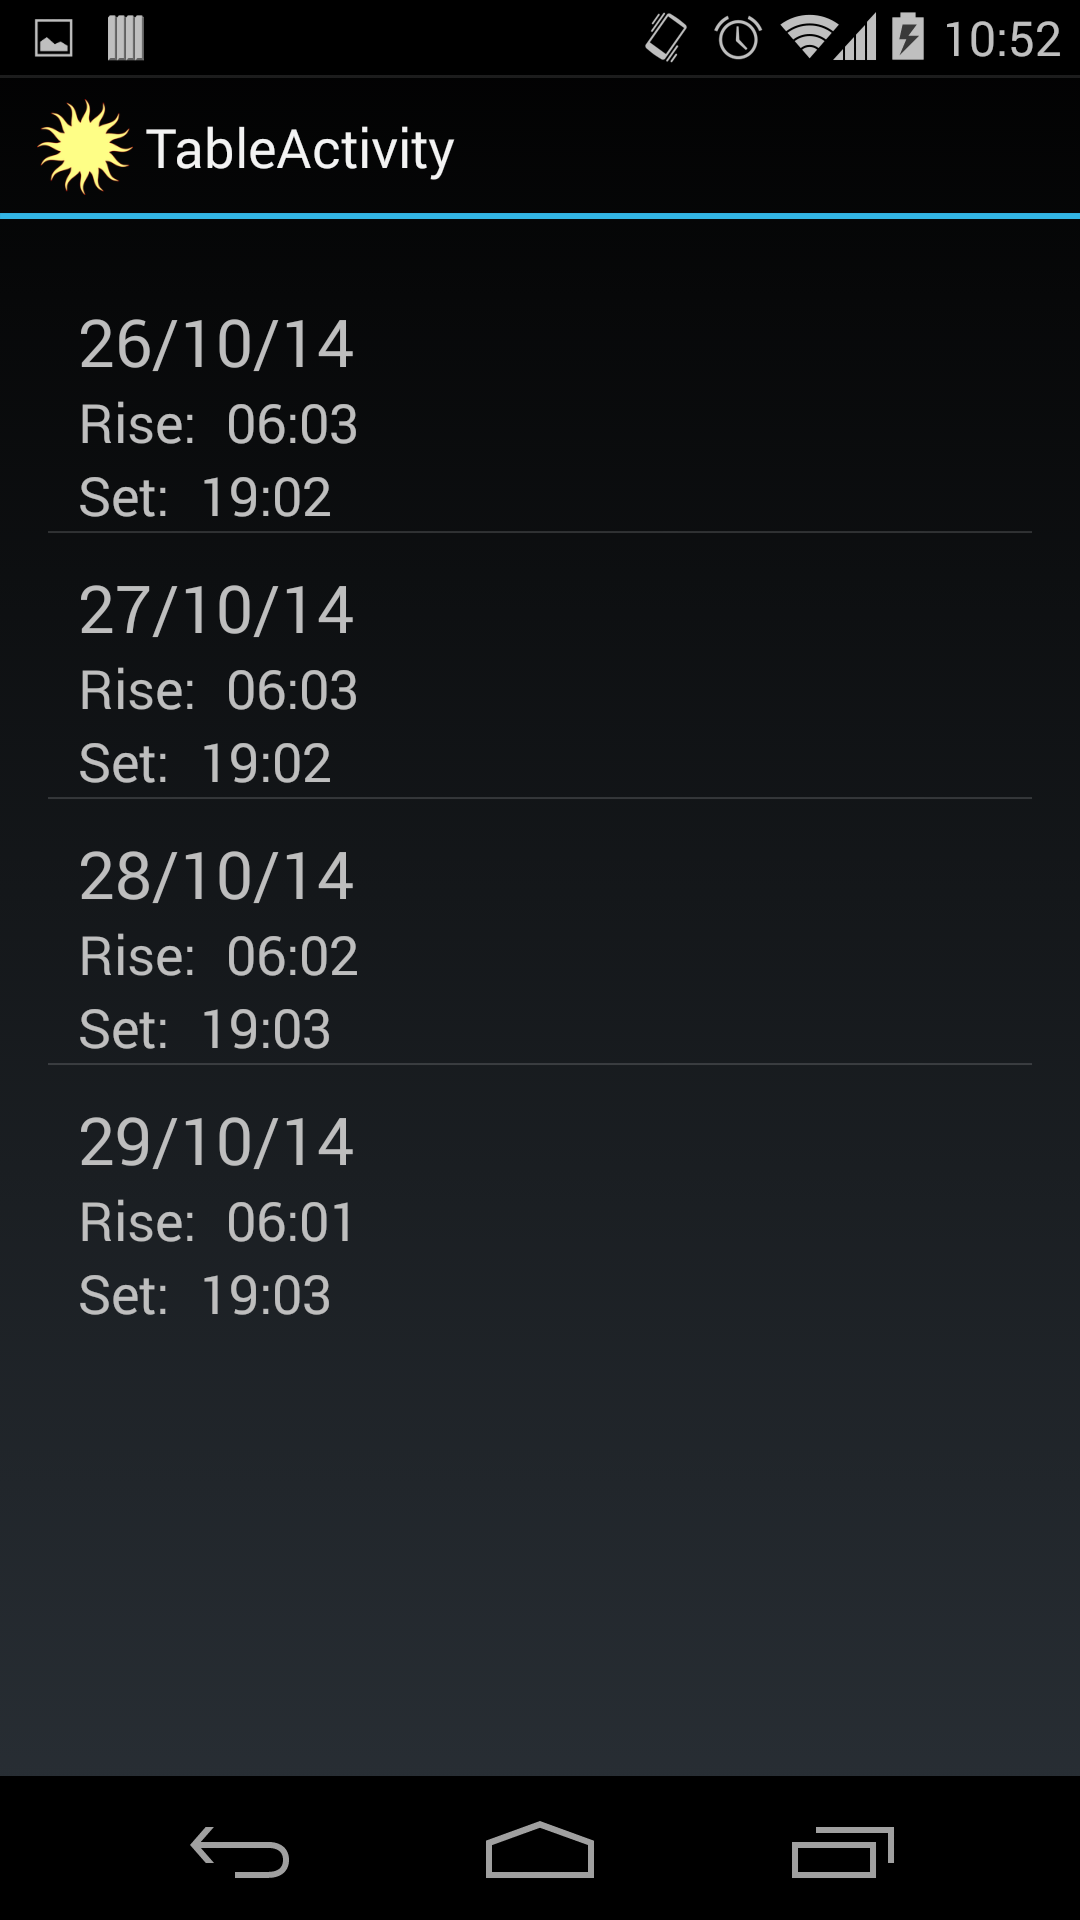
\includegraphics[width=5cm]{images/table.png}}
}\\
\end{figure}

\begin{figure}[H]
\centering{
	\fbox{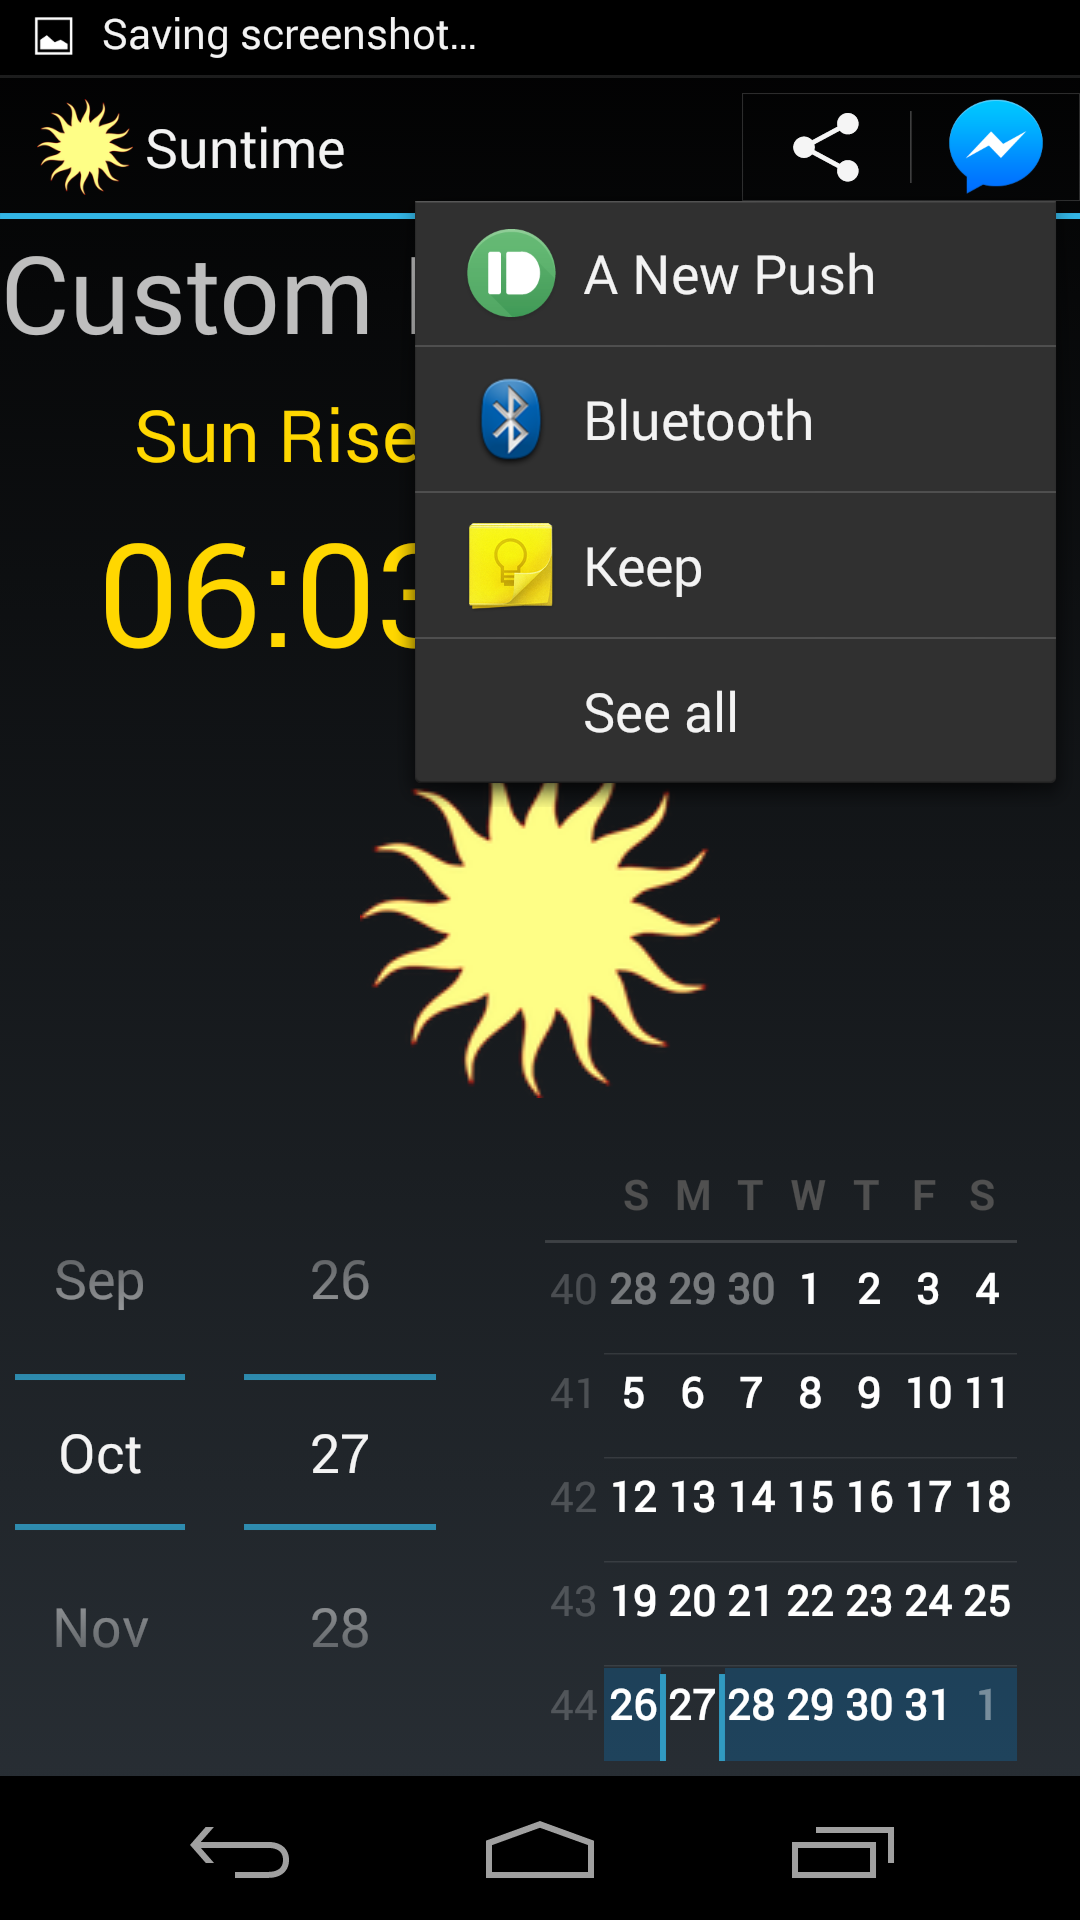
\includegraphics[width=5cm]{images/share.png}}
}\\
\end{figure}
\begin{landscape}
\subsection{Source}
\subsubsection{MainActivity}
\inputminted[firstline=17, lastline=82]{java}{../../Apps/FinalSuntime/app/src/main/java/au/net/danielparker/suntime/ui/MainActivity.java}

\subsubsection{CustomFragment}
\inputminted[firstline=28, lastline=89]{java}{../../Apps/FinalSuntime/app/src/main/java/au/net/danielparker/suntime/ui/CustomFragment.java}


\end{landscape}
\end{document}
